\documentclass[11pt,preprint, authoryear]{article}

\pagestyle{plain}

\usepackage{lmodern}

% spacing passed through from .Rmd doc
\usepackage{setspace}
\setstretch{1.5}

% Wrap around which gives all figures included the [H] command, or places it "here". This can be tedious to code in Rmarkdown.
\usepackage{float}
\let\origfigure\figure
\let\endorigfigure\endfigure
\renewenvironment{figure}[1][2] {
    \expandafter\origfigure\expandafter[H]
} {
    \endorigfigure
}

\let\origtable\table
\let\endorigtable\endtable
\renewenvironment{table}[1][2] {
    \expandafter\origtable\expandafter[H]
} {
    \endorigtable
}

\usepackage{ifxetex,ifluatex}
\usepackage{fixltx2e} % provides \textsubscript
\ifnum 0\ifxetex 1\fi\ifluatex 1\fi=0 % if pdftex
  \usepackage[T1]{fontenc}
  \usepackage[utf8]{inputenc}
\else % if luatex or xelatex
  \ifxetex
    \usepackage{mathspec}
    \usepackage{xltxtra,xunicode}
  \else
    \usepackage{fontspec}
  \fi
  \defaultfontfeatures{Mapping=tex-text,Scale=MatchLowercase}
  \newcommand{\euro}{€}
\fi

\usepackage{amssymb, amsmath, amsthm, amsfonts}

\DeclareMathSizes{24}{26}{22}{22}

\usepackage[round]{natbib}
\bibliographystyle{natbib}
\def\bibsection{\section*{References}} %%% Make "References" appear before bibliography
\usepackage{longtable}

% set margins
\usepackage[left=3.5cm, right=2cm, top=30mm ,bottom=2cm, includefoot]{geometry}
\usepackage{fancyhdr}
\usepackage[bottom, hang, flushmargin]{footmisc}
\usepackage{graphicx}
\numberwithin{equation}{section}
\numberwithin{figure}{section}
%\numberwithin{table}{section} % commented out because it messes up table numbering
\setlength{\parindent}{0cm}
\setlength{\parskip}{1.3ex plus 0.5ex minus 0.3ex}
\usepackage{textcomp}
\renewcommand{\headrulewidth}{0pt}

\usepackage{array}
\newcolumntype{x}[1]{>{\centering\arraybackslash\hspace{0pt}}p{#1}}

\usepackage{hyperref}
\hypersetup{breaklinks=true,
            bookmarks=true,
            colorlinks=true,
            citecolor=blue,
            urlcolor=blue,
            linkcolor=blue,
            pdfborder={0 0 0}}
						
\urlstyle{same}  % don't use monospace font for urls
\setlength{\parindent}{0pt}
\setlength{\parskip}{6pt plus 2pt minus 1pt}
\setlength{\emergencystretch}{3em}  % prevent overfull lines
\setcounter{secnumdepth}{5}

% Use protect on footnotes to avoid problems with footnotes in titles
\let\rmarkdownfootnote\footnote%
\def\footnote{\protect\rmarkdownfootnote}
\IfFileExists{upquote.sty}{\usepackage{upquote}}{}

% pass through extra packages specified by user
\usepackage{bm}

%%%%%%%%%%%%%%%%%%%%%%%%%%%%%%%%%%%%%%%%%%%
%%%%%%%%%%%%%%%%%% EDIT TITLE %%%%%%%%%%%%%%%%%%
%%%%%%%%%%%%%%%%%%%%%%%%%%%%%%%%%%%%%%%%%%%

% change title format to be more compact
\usepackage{titling}

% create subtitle command for use in maketitle
\newcommand{\subtitle}[1]{
  \postauthor{
    \begin{center}\large#1\end{center}
    }
}

\setlength{\droptitle}{-1em}
\pretitle{\vspace{\droptitle}\centering\Huge}
\posttitle{\par\vskip 5.5em}

\title{
{\scshape\Large Department of Statistics 2019}\\
{\vskip 2.5em \scshape Predicting Community Engagement with Questions Across Online
Question-Answer Fora}\\
%{\includegraphics{lse.png}} % if you want to include LSE logo
}

\preauthor{\centering\LARGE}
\postauthor{\par\vskip 4em}

\author{Candidate Number: 10140}
\subtitle{\vspace{4em} Submitted for the Master of Science, London School of Economics,
University of London} % comment this out and you get *Missing \begin{document}*

\predate{\centering\Large}
\postdate{\par}

\date{\scshape August 2019}

\usepackage{color}
\usepackage[usenames,dvipsnames,svgnames,table]{xcolor}
\usepackage{hyperref}
\hypersetup{
     colorlinks = true,
     citecolor = gray
}

\usepackage{tocloft}

\renewcommand{\cftsubsecfont}{\normalfont\hypersetup{linkcolor=black}}
\renewcommand{\cftsubsecafterpnum}{\hypersetup{linkcolor=black}}

%%%%%%%%%%%%%%%%%%%%%%%%%%%%%%%%%%%%%%%%%%%
%%%%%%%%%%%%%%%% BEGIN DOCUMENT %%%%%%%%%%%%%%%%
%%%%%%%%%%%%%%%%%%%%%%%%%%%%%%%%%%%%%%%%%%%

\begin{document}

% Header and Footers
\pagestyle{fancy}
\chead{}
\rhead{}
\lfoot{}
\rfoot{} 
\lhead{}
%\rfoot{\footnotesize Page \thepage\ } % "e.g. Page 2"
\cfoot{\footnotesize \thepage\\}

% i, ii, iii etc. page numbering
\pagenumbering{roman}

\maketitle

\thispagestyle{empty}

\clearpage

\setcounter{page}{1}

% table of contents, list of figures and tables
\renewcommand{\contentsname}{Table of Contents}
\hypersetup{linkcolor=black}
\tableofcontents
\newpage
\hypersetup{linkcolor=black}
\listoffigures
\newpage
\hypersetup{linkcolor=black}
\listoftables
\hypersetup{linkcolor=black}
\newpage

\section*{Summary}

Formulating constructive questions and receiving answers to these
questions is not only a key part of how we learn, but also to scientific
and human progress. The advent of the world wide web and the
technologies it has provided us has given us an unprecendented ability
to engage with and learn from the world and while substantial attention
has been dedicated to finding correct answers (just ask Google),
comparitively less has been devoted to how we can improve the
constructiveness of our questions. One online setting where relevant and
well-researched questions is of particular importance is online
question-answer (Q\&A) communities, where professional resources are
scarce and questions are in abundance. This research aims to address
this challenge of information overload by the extent of community
engagement with new questions submitted to various onlinw communities.
In this way, questioners on online educational fora can be nudged to
enhance the ``signal'' of their questions before adding demand to these
communities, thereby improving the functioning and efficiency of these
platforms. I build on work done on questions in Q\&A communities by
constructing a model to predict on a metric comprising of the
community-granted score and viewcount of questions in a number of
diverse Q\&A communities. Using only the textual variables (i.e.~the
question title and body) available at the time a user submits a question
to a forum, I am able to \textbf{engineer features and build models}
that improve upon baselines by up to \textbf{so-much-\%}. I further
conclude, from the variation of performance of these models across fora,
that \textbf{communities are diverse?}

\clearpage

% 1, 2, 3 etc. page numbering
\pagenumbering{arabic}

\newpage

\section{\texorpdfstring{Introduction
\label{Intro}}{Introduction }}\label{introduction}

Modern interpersonal communication technologies made possible by the
internet have afforded us an exceptional level of connection and
engagement with the world. Billions of individuals now interact online
daily, not only with people that they know, but with strangers millions
of miles away. There are now a multitude of online platforms and
knowledge-sharing communities such as Yahoo! Answers, Quora, the
StackExchange family and Massive Online Open Courses (MOOCs) where users
seek discussions on and answers to complex questions that search engines
are yet unable to fully address.

This research focuses on online social question-and-answer (Q\&A) fora,
which are platforms for community knowledge-sharing and are particularly
prone to the problem of ``information overload'' where cascades of new
questions far outweigh the few expert resources available. \textbf{A
substantial amount of research has been done on Q\&A sites, however the
focus has been on identifying expert users and high quality answers and
considerably less attention has been given to questions, despite their
being the entry point for every interaction in the community}.

I plan to address this issue of information overload in online Q\&A
communities by building a model to predict community engagement with
questions. This research thus has a concrete application to the real
world: providing these predictions to questioners in real-time can
encourage them to improve the ``signal'' of their questions before they
submit new questions and add demand to the resources of a community.
\textbf{In this way, it is hoped that the functioning and evolution of
these online communities can be improved.}

The broad research question can therefore be defined as the following:

\begin{center}
\emph{To what extent can community engagement with questions in online Q\&A communities be accurately captured and predicted?}
\end{center}

I draw heavily on and critique prior research done on Q\&A platforms by
Ravi \emph{et al.} (2014) and analyse question content from the
\href{https://stackexchange.com/sites\#}{StackExchange} family of Q\&A
communities. These Q\&A fora have a voting mechanism whereby registered
community-members can signal how much value specific questions add to
the community and it is precisely this metric which I identify as
community engagement and aim to predict \textbf{and evaluate using
root-mean-square error (RMSE)}. The inherent assumptions for the problem
as it is stated are that: questions are heterogeneous in their
formulation (along lines of clarity, showing prior research and
community-relevance) and that the voting mechanism of a community for a
question captures this heterogeneity.

This research goal thus takes the form of quantitative prediction task
rather than qualitative, causal or inferential analysis. I leave it to
further research to address the \emph{how} and \emph{why} of community
engagement on online Q\&A communities, rather than just the \emph{what}
that is explored here. I believe that the fact that this research aims
to predict a community-provided measurement of online engagement, has a
direct real-life application and will be implemented on \textbf{diverse
communities makes it the first of its kind.}

\textbf{My results are this this and that, and I conclude that the LDA
topic model is not universally effective as Ravi \emph{et al.} (2014)
claimed.}

Previous work in the field of questions in online Q\&A fora will now be
discussed. This is followed by a discussion of the data, exploration of
the concerned variables visually, a description of the model used, and
presentation and discussion of the results. Finally, some concluding
remarks and recommendations for areas of further research are made.

\newpage

\section{\texorpdfstring{Literature Review
\label{Lit}}{Literature Review }}\label{literature-review}

\color{blue}

Much work has gone into investigating online Q\&A communities. Research
has looked at answer quality (Jeon \emph{et al.}, 2006; Shah and
Pomerantz, 2010; Tian, Zhang and Li, 2013), behaviour of community
experts (Riahi \emph{et al.}, 2012; Sung, Lee and Lee, 2013) and
question-asker satisfaction (Liu, Bian and Agichtein, 2008). Also, a
common framework for engagement in Q\&A communities is the optimisation
of matching questions and community experts (Li and King, 2010; Li, King
and Lyu, 2011; Zhou, Lyu and King, 2012; Shah \emph{et al.}, 2018), or
recommending questions in line with answerers' interests (Wu, Wang and
Cheng, 2008; Qu \emph{et al.}, 2009; Szpektor, Maarek and Pelleg, 2013).

I choose to focus on questions, not only because they have received far
less attention in the literature, but because question quality impacts
answer quality (Agichtein \emph{et al.}, 2008) and because they are
trivially the initial touch-point of a community/questioner interaction.
It is highly likely therefore that increasing positive community
engagement will improve how these communities function and evolve.

Since community engagement and question quality can be seen as two sides
of the same coin (``good'' questions leading to favourable community
engagement), this research corresponds to a body of work on capturing
question quality in online question-answer communities which I briefly
discuss next. Note that while I consider community engagement a more
accurate definition of what the following literature measures, I refer
to ``question quality'' instead of community engagement to aid the
discussion.

Recent work (Agichtein \emph{et al.}, 2008; Bian \emph{et al.}, 2009; Li
\emph{et al.}, 2012) attempted to model question quality using
\href{http://answers.yahoo.com}{Yahoo! Answers}, however this dataset
lacks objective and definitive measures for question quality. The data
that I will be using on the other hand is richer in that there a
numerous proxies for question quality/community engagement available for
large sets of observations. Most importantly, these variables are
derived directly from the data rather than labeled manually, which
enables a more objective, automatic and principled characterisation of
the variable of interest.

One paper that made strides in classifying and predicting what they
assume to be question quality is Ravi \emph{et al.} (2014). Using latent
topics extracted from Latent Dirichlet Allocation models on question
content, they predict ``question quality'' with accuracy levels of 72\%
for the computer coding StackExchange community, StackOverflow.

Ravi \emph{et al.} (2014) decide on using a question's \texttt{Score} as
an indicator of question quality. I question this assumption and put
forth the notion that a question's \texttt{Score} better characterises
community engagement, since I believe it is difficult to define
``quality'' subjectively owing to communities valuing different facets
of questions (i.e.~closed-end for natural sciences or
discussion-promoting in the social sciences). I thus characterise it as
such and also use it as a response variable. This brings me to the aim
of this paper, which is to critique and build on how to use the
\texttt{Score} variable to label questions as attracting positive or
negative community engagement.

\subsection{Question Quality - All before
Ravi}\label{question-quality---all-before-ravi}

Intuitively, question quality and community engagement are two sides of
the same coin - high-quality questions assuredly lead to positive
community engagement. As will be argued later, I consider community
engagement a more robust characterisation of what is being measured in
the following literature, however I will refer to ``question quality''"
rather than community engagement for the sake of this discussion.

Question quality has been investigated using the online question-answer
community \href{http://answers.yahoo.com}{Yahoo! Answers} (Agichtein
\emph{et al.}, 2008; Bian \emph{et al.}, 2009; Li \emph{et al.}, 2012),
but a considerable limitation of this dataset is that it lacks objective
and clear-cut metrics for question quality. To address this, Agichtein
\emph{et al.} (2008) use semantic features (punctuation, typos, lexical
complexity etc.) to define quality questions, Bian \emph{et al.} (2009)
make use of manual labels to identify quality in a sample of 250
questions, and Li \emph{et al.} (2012) use a combination of tag count,
answer count and time-to-first-answer along with domain expert and
author judgement to ascertain ground truth.

Fortunately, the StackExchange fora that I will explore are richer
datasets in the sense that a greater number of proxies for question
quality and community engagement are available. More importantly, these
metrics are more objective as they are derived from the data itself
rather than manual human labeling. In this way, it is also possible to
``automatically'' define question quality with a
robust\footnote{The key issue being the assumptions made and the manner in which this labeling occurs}
response variable, vastly increasing the number of ground truth cases.

Another substantial difference that has evolved over time in the
question-quality literature is the chosen predictive model. Previous
work (Agichtein \emph{et al.}, 2008; Bian \emph{et al.}, 2009; Anderson
\emph{et al.}, 2012; Li \emph{et al.}, 2012) chose to use features such
as the question category, lexical properties of the question (length,
level of misspelling, words-per-sentence) and question-asker's
reputation for prediction.

By ignoring words, topics and other inherent question content and
focusing instead on features of the question-asker, users asking
questions for the first time would be largely ignored by models of this
kind. This is directly opposed to my specific goal of predicting how
communities will engage with all users, especially new and inexperienced
users who are likely to not have their questions answered at all, let
alone positively. For my modeling task, I therefore only focus on
explanatory features derived from the contents of questions, not user
attributes, history or other data.

\subsection{Question-Answer Communities - Others then
Ravi}\label{question-answer-communities---others-then-ravi}

A substantial amount of research has investigated question-answer
communities. Work has been done on quality of answers (Jeon \emph{et
al.}, 2006; Shah and Pomerantz, 2010; Tian, Zhang and Li, 2013),
questioner satisfaction (Liu, Bian and Agichtein, 2008) and behaviour of
expert users (Riahi \emph{et al.}, 2012; Sung, Lee and Lee, 2013). Work
on question-answer communities has also often been placed in the
framework of a matching process where the goal is optimising the routing
of user questions to expert resources (Li and King, 2010; Li, King and
Lyu, 2011; Zhou, Lyu and King, 2012; Shah \emph{et al.}, 2018), or
routing questions according to answerers' interests as a recommendation
system (Wu, Wang and Cheng, 2008; Qu \emph{et al.}, 2009; Szpektor,
Maarek and Pelleg, 2013).

My approach differs to this previous work in two main aspects. Firstly,
rather than focusing on answer or user characteristics, I focus on
questions. As Agichtein \emph{et al.} (2008) show, question quality can
significantly impact answer quality. Trivially, questions also serve as
the initial event in the question-answering process, upon which all
community engagement follows. Thus, maximising the positive community
engagement of questions will most certainly enhance the functioning and
development of a community.

The second difference is the framework in which I place the research. I
steer clear of the systems-based framework of optimising
matching/routing mechanisms and instead centralise how users can be
nudged to improve aspects of their question before exerting demand on
expert resources. This framework coincides strongly with a large body of
research on codifying question quality in question-answer communities,
and so this is discussed next.

\textbf{Why I choose a continuous response}

\subsection{\texorpdfstring{Topic Modeling
\label{model_lit}}{Topic Modeling }}\label{topic-modeling}

Focusing on the textual content of questions alone leads me to a
discussion on how this text will be modeled. Bayesian models have gained
popularity in solving diverse structured prediction tasks in Natural
Language Processing (NLP) (Chiang \emph{et al.}, 2010), and Latent
Dirichlet Allocation (LDA) (Blei, Ng and Jordan, 2003) is a form of
topic modeling where generative Bayesian models are applied to documents
to model hidden topics as a probability distribution over words. LDA can
thus be used to uncover the underlying semantic structure of documents
and infer topics associated with these documents.

Indeed, Ravi \emph{et al.} (2014) show that using latent topics derived
from LDA modeling allows for powerful prediction (accuracy scores of up
to 72\%) of ``question quality'' using the coding question-answer site,
\href{https://stackoverflow.com}{StackOverflow}. My analysis will mirror
not only the modeling methodology of Ravi \emph{et al.} (2014), but also
critique and build on the methodology they use to define their metric
for question quality.

The final predictive model that Ravi \emph{et al.} (2014) employ is
based on a model proposed by Allamanis and Sutton (2013), who themselves
analysed StackOverflow questions but did not use their model to predict
``question quality''. Allamanis and Sutton (2013) use LDA models on
three tiers: First across the entire question body, secondly on the code
chunks in the body, and lastly on the body with noun phrases removed.
Ravi \emph{et al.} (2014) on the other hand choose the following three
levels over which to model latent topics: Globally to capture topics
over the entire question content, locally to capture sentence-level
topics, and a Mallows model (Fligner and Verducci, 1986) global topic
structure to enforce structural constraints on the sentence topics in
questions. This is the same model that I will employ in task two of my
research question.

\newpage 

\color{black}

\section{\texorpdfstring{Methodology
\label{Method}}{Methodology }}\label{methodology}

\subsection{\texorpdfstring{Data \label{Data}}{Data }}\label{data}

The \href{https://stackexchange.com/sites\#traffic}{StackExchange}
family of online Q\&A fora are a diverse range of over 170 community
websites ranging from vegetarianism to quantum computing to bicycles,
and a rich amount of data from all the communities is publicly available
in XML files compressed in 7-Zip format at
\href{http://archive.org/download/stackexchange}{archive.org}.

The \textbf{five} datasets that I chose to analyse are displayed in
table \ref{tab:fora}, along with their descriptions.

\footnotesize

\begin{longtable} {@{} cccp{9cm} @{}}
\caption{\textbf{Datasets}}
\label{tab:fora}\\ \hline \hline
Forum & Questions & Answers & Description \\ 
\hline
StackOverflow & 18m & 27m & Q\&A for professional and enthusiast programmers \\
Math & 1.1m & 1.5m & Q\&A for people studying math at any level \\
SuperUser & 415k & 601k & Q\&A for computer enthusiasts and power users \\ 
Russian StackOverflow & 273k & 310k & Q\&A for programmers (Russian) \\ 
English & 106k & 249k & Q\&A for linguists, etymologists, English language enthusiasts \\ 
Buddhism & 5.7k & 19k & Discussions on Buddhist philosophy, teaching and practice \\
Economics & 7.7k & 9.9k & For those studying, teaching, researching and applying economics/econometrics \\
Fitness & 8.2k & 16k & Q\&A for athletes, trainers and physical fitness professionals \\ 
Health & 5.6k & 4.5k & For professionals in the medical and allied health fields \\ 
Interpersonal & 3.1k & 13k & Q\&A for anyone wanting to improve their interpersonal skills \\ 
\hline \hline
\end{longtable}

\normalsize

\textbf{I extracted the full number of questions from each forum for
analysis, resulting in a total number of questions of \emph{so-much} },
with the following variables of interest per community:

\setstretch{0.65}

\begin{itemize}
\item
  \texttt{Score}: The difference between registered-user attributed
  up-votes and down-votes for a question
\item
  \texttt{ViewCount}: A counter for the number of page views the
  question receives (by both registered and non-registered users)
\item
  \texttt{Title}: The text of the question title
\item
  \texttt{Body}: The text of the question body
\item
  \texttt{CreationDate}: A datetime variable indicating when the
  question was initially posted
\end{itemize}

\setstretch{1.25}

The date ranges for questions from each community are as follows:

Buddhism: 2014-06-17 to 2019-03-02

Economics: 2014-11-18 to 2019-03-03

Fitness: 2011-03-01 to 2019-03-03

Health: 2015-03-31 to 2019-03-02

Interpersonal: 2017-06-27 to 2019-03-02

I now move onto some noteworthy aspects of the data.

\subsection{\texorpdfstring{Noteworthy elements
\label{noteworthy}}{Noteworthy elements }}\label{noteworthy-elements}

\textbf{A discussion of the underlying functioning of StackExchange
sites is necessary to gain insight to abilities and limitations of the
research goal.} While questions on all StackExchange sites are open to
the public, posting a question in a community requires registration with
an email address and a username. Once registered, users start with a
\emph{reputation} level of 1
(\url{https://meta.stackexchange.com/questions/7237/how-does-reputation-work}).
The reputation levels key to my analysis are laid out as follows:

\setstretch{0.65}

\begin{itemize}
\item
  15: Users are allowed to ``up-vote'' questions and answers
\item
  125: Users can ``down-vote'' questions and answers
\item
  1000: Users can edit any question or answer.
\end{itemize}

\setstretch{1.25}

A number of complexities are created by the structure of the websites.
First of all, the contrasting reputation levels for up- and down-voting
privileges (15 and 125 respectively) lead to a \texttt{Score} variable
that is highly negatively skewed and thus questions are more likely to
have a higher \texttt{Score}, thus making it appear as if more questions
are highly value in the community than could actually be. Table
\ref{tab:score_table} below confirms this:

\footnotesize

\begin{longtable}[htbp] {@{} lccc @{}} 
\caption{\textbf{Score Distribution}} 
\label{tab:score_table} \\
\hline \hline
\textbf{Score} &  \textbf{<0} &  \textbf{=0} &  \textbf{>0} \\
\hline \hline
\% of questions Economics    &              0 &              0 &                0 \\
\% of questions Buddhism      &              0 &              0 &                0 \\
\% of questions Fitness       &              0 &              0 &                0 \\
\% of questions Health        &              0 &              0 &                0 \\
\% of questions Interpersonal &              0 &              0 &                0 \\
\hline \hline
\end{longtable}\begin{center} Source: Own calculations in PySpark\end{center}

\normalsize

\textbf{This does not serve much of an issue for our model however,
because the \texttt{Score} variable is continuous and thus can just view
that as a range where it is easy to get percentiles of new questions to
see how they rank versus old ones.}

One challenge in just considering the \texttt{Score} as the target
variable alone, is that it does not take into account what
\emph{proportion} of users have decided to vote - i.e.~the percentage of
voters that decided to up-vote a question could be small in comparison
to the total amount of users that viewed the question.

Thus as As Ravi \emph{et al.} (2014) note suggest, a natural improvement
upon only using the \texttt{Score} variable would be to consider the
\texttt{Score} variable normalised by \texttt{ViewCount}, i.e.
\texttt{Score}/\texttt{ViewCount}. This raises a further issue however,
since the fact that all questions are open to the public, not everyone
who views a question (and thus adds to the \texttt{ViewCount}) has the
ability to vote on the question (i.e.~non-registered members, those
registered who cannot vote due to a reputation level below 15). In order
to address this issue in their own analysis, Ravi \emph{et al.} (2014)
decide on a minimum \texttt{ViewCount} threshold so that they are more
confident that their final dataset contains questions that have been
viewed by qualifying users that can vote. I opt not to discard questions
below a certain \texttt{ViewCount} in my analysis, since I believe there
is no material manner in which to ascertain if questions have been
viewed by qualifying or non-qualifying users, despite how low their
\texttt{ViewCount}.

Lastly, a possible confounding factor is that questions can be edited,
not only by the original poster, but by anyone with a level of
reputation of 1000 or more. General cross-community guidelines for
editing include addressing grammar and spelling issues, clarifying
concepts, correcting minor mistakes, and adding related resources and
links. The concern here is that users could vote, comment and answer on
substantially different questions over time as a question is edited from
it's original form. \textbf{The simplifying assumption that I make here
is that most edits, if any at all, would happen quickly as moderators
are made aware of offending questions and thus the majority of views and
votes would happen on final, edited questions. I therefore choose final
edited question content to predict on.}

\textbf{It seems that ViewCount and Score could be working
counteractively at times, since a high viewcount and low score could
mean high outside community interaction, whereas the opposite indicates
high inside community interaction. I focus on within community
interaction.}

\subsection{Preprocessing and Exploratory
Analysis}\label{preprocessing-and-exploratory-analysis}

The PySpark code for the processing and modelling of the data done can
be found
\href{https://github.com/BCallumCarr/msc-lse-thesis/tree/master/01-python-code}{here}.
I downloaded the full data from the 5 selected fora, decompressed the
7-Zip files and converted the XML files into
\href{https://parquet.apache.org}{Parquet} format.

\textbf{Table \ref{tab:bestworst} displays the titles of a selection of
``best'' and ``worst'' questions across fora according to the final
response variable \texttt{Score}/\texttt{ViewCount} (the best questions
have positive \texttt{Scores} whereas the worst have negative
\texttt{Scores}).}

\footnotesize

\begin{longtable} {@{} cccp{11cm} @{}}
\caption{\textbf{Best and Worst Fora Questions According to Score/ViewCount}}
\label{tab:bestworst}\\ \hline \hline
\textbf{Forum} & \textbf{Score} & \textbf{ViewCount} & \textbf{Title} \\ 
\hline
Buddhism & 13 & 176 & What are the texts that contain words which can be attributed directly to the Buddha? \\
\hline
Economics & -9 & 102 & Has anyone made a successful economic prediction more than once? \\
\hline
Health & 14 & 95 & In which order to put on a mask, a gown and to disinfect when visiting a hospital patient? \\ 
\hline
Fitness & -5 & 201 & What is the best way to gain size in ankle area \\ 
\hline
Interpersonal & 24 & 1054 & How can I notice if someone is speaking with sarcasm or irony? \\ 
\hline
Interpersonal & -9 & 1327 & How can I tell if family members consider my unvaccinated kids a threat? \\ 
\hline
Spanish & 20 & 330 & Is the use of @ instead of 'a' or 'o' in order to refer to both masculine and femenine accepted? \\ 
\hline \hline
\end{longtable}\begin{center} Source: Own calculations in Python.\end{center}

\normalsize

\textbf{Table \ref{tab:bestworst} appears to show that questions that
are considered the ``best'' tend to be honest and discussion-promoting,
whereas the ``worst'' questions are often sarcastic and probably not
genuinely looking for an answer - the questions from the Economics and
Fitness fora illustrate this. Social norms also appear to play a strong
part, since the ``worst'' question on the Interpersonal forum eludes to
children being unvaccinated, which I assume would upset many individuals
on the forum and lead to lowest \texttt{Score} per \texttt{ViewCount}
for that forum.}

Some descriptive graphs of the initial variables are displayed in figure
\ref{fig:desc}. Here we see a number of differences across fora.
\textbf{StackOverflow} has by far the highest number of questions, no
doubt as a result of it being the first and oldest StackExchange site,
followed by Mathematics. We see that \ldots{}.

\renewcommand{\thefigure}{\arabic{figure}}

\footnotesize

\begin{figure}
\caption{\textbf{Fora Descriptive Statistics}}
\label{fig:desc}
\begin{minipage}{1\textwidth}

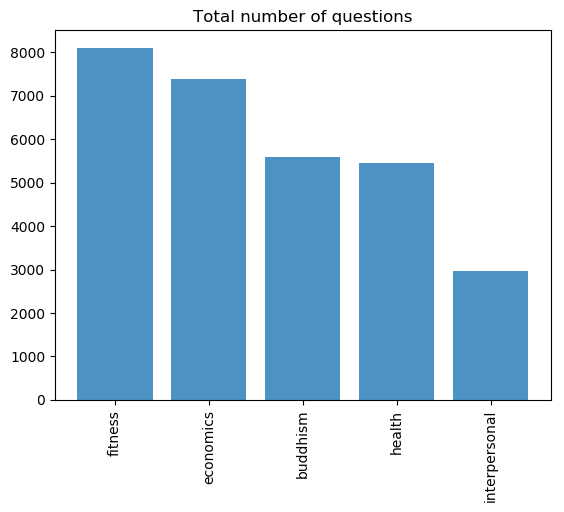
\includegraphics[width=0.32\linewidth]{../../01-python-code/00-workspace/01-graphs/post-counts-bar-graph} 
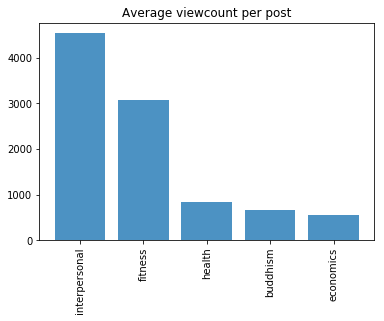
\includegraphics[width=0.32\linewidth]{../../01-python-code/00-workspace/01-graphs/ave-views-bar-graph} 
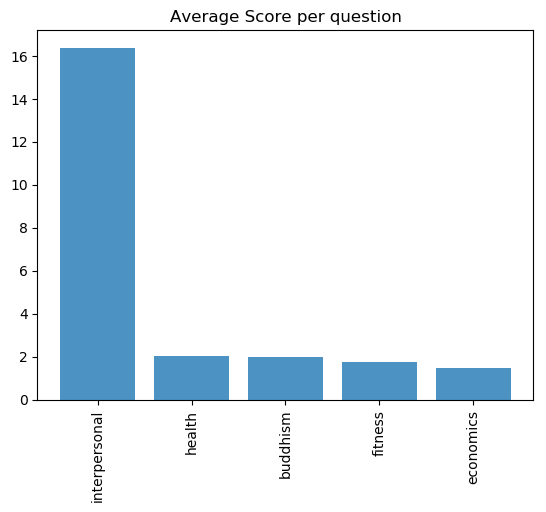
\includegraphics[width=0.32\linewidth]{../../01-python-code/00-workspace/01-graphs/ave-score-bar-graph} 
\\ \centering
{\footnotesize Source: Own calculations in Python.}
\end{minipage}
\end{figure}

\normalsize

\textbf{Graph response variable score to see skewness}

It looks like the claim in Ravi \emph{et al.} (2014) that their model
should work across disciplines is on thin ice, but we will look deeper
into this with the modelling results.

\textbf{Talk about assumptions of response variable?}

\subsection{\texorpdfstring{Model \label{Model}}{Model }}\label{model}

\color{black}

I split that set of questions, \(Q\), into a training set
\(Q_\text{train}\) and testing set \(Q_\text{train}\) using a point in
time to mimic the reality of employing this tool at a certain point in
time with historical training data. With the chosen date of
\textbf{1/1/2017}, the ratio of \(Q_\text{train}\) to \(Q_\text{train}\)
are \ldots{}\ldots{}. for \ldots{}\ldots{}\ldots{} respectively.

\textbf{This addresses something that has not been considered in the
literature and introduces a temporal element into the analysis. While I
do not employ time-series models, I leave it to further research to
incorporate a way to ``remember'' which questions are good, so that in
future there are no duplicates.}

I employ a simple regularised regression with the \texttt{Body} and
\texttt{Title} as inputs from questions \(q_i\) out of
\(Q_\text{train}\), i.e.~the learning goal is to find a coefficient
vector \(\bm{\beta}\) that minimises the Root Mean Squared Error:

\begin{align} \label{rmse}
\underset{\bm{\beta}}{\text{minimise}} \quad \sqrt{ \frac{1}{|Q_\text{train}|} \sum_{ q_{i} \in Q_{\text{train}} } ( y_i - {\bm{\beta}\phi(\bm{x'}_i}) )^2 + \lambda \bm{\beta}\bm{\beta'} }
\end{align}

The \(y_i\) is the true value of the response variable,
\texttt{Score}/\texttt{ViewCount}, and \(\bm{\beta}\phi(\bm{x'}_i)\) is
the predicted response. \(\phi(\cdot)\) is a function on the features,
and leads to the feature engineering, of which lda is discussed in
section \ref{lda}. \(\lambda\) is the regularisation parameter
\ldots{}\ldots{}.

I use the \texttt{pyspark.sql.mllib} package in PySpark and inherent
online LDA learning framework to solve the optimisation problem
\ref{rmse}.

I use 2-fold cross validation - 2 because increasing the number of folds
did not lead to large gains in RMSE reduction, and also drastically
increased computation time.

\subsection{Feature Engineering}\label{feature-engineering}

A number of preprocessing steps was then applied to the question
\texttt{Body} and \texttt{Title} - HTML parsing for the question content
in the \texttt{Body} variable, tokenisation, removal of English
stopwords and Russian stopwords for Russian StackOverflow and stemming
of tokens.

\section{\texorpdfstring{Results
\label{Results}}{Results }}\label{results}

\footnotesize

\begin{longtable}[htbp] {@{} lccc @{}} 
\caption{\textbf{Constant Mean Model}} 
\label{tab:mean_model} \\
\hline \hline
\textbf{Forum} &  \textbf{Train RMSE} &  \textbf{Test RMSE} &  \textbf{Time (s)} \\
\hline \hline
Economics     &              0.026557 &              0.037792 &                0.93 \\
Buddhism      &              0.014359 &              0.015749 &                0.75 \\
Fitness       &              0.012305 &              0.020767 &                0.41 \\
Health        &              0.035457 &              0.040167 &                0.67 \\
Interpersonal &              0.004935 &              0.008395 &                0.56 \\
\hline \hline
\end{longtable}\begin{center} Source: Own calculations in PySpark\end{center}

\normalsize

\footnotesize

\begin{longtable}[htbp] {@{} lcccc @{}} 
\caption{\textbf{Viewcount Model}} 
\label{tab:vc_model} \\
\hline \hline
\textbf{Forum} &  \textbf{Train RMSE} &  \textbf{Test RMSE} &  \textbf{Test Gain (\%)} &  \textbf{Time (s)} \\
\hline \hline
Economics     &             0.026223 &          0.037722 &              0.185 &               5.96 \\
Buddhism      &             0.014088 &          0.015799 &             -0.317 &               5.23 \\
Fitness       &             0.012161 &          0.020627 &              0.674 &               4.32 \\
Health        &             0.035242 &          0.040102 &              0.162 &               4.07 \\
Interpersonal &             0.004805 &          0.008177 &              2.597 &               4.09 \\
\hline \hline
\end{longtable}\begin{center} Source: Own calculations in PySpark\end{center}

\normalsize

\footnotesize

\begin{longtable}[htbp] {@{} lcccccc @{}} 
\caption{\textbf{Tokens Model}} 
\label{tab:vc_model} \\
\hline \hline
\textbf{Forum} &  \textbf{Train RMSE} &  \textbf{Test RMSE} &  \textbf{Test Gain (\%)} &  \textbf{Time (s)} & \textbf{Elastic Param} &  \textbf{Reg'tion Param} \\
\hline \hline
Economics     &          0.026446 &       0.037769 &           0.061 &          606.66 &             0.001 &             1.000 \\
Buddhism      &          0.014281 &       0.015740 &           0.057 &          385.50 &             1.000 &             0.001 \\
Fitness       &          0.012305 &       0.020767 &          -0.000 &          571.22 &             0.001 &             1.000 \\
Health        &          0.035030 &       0.040057 &           0.274 &          374.23 &             0.001 &             1.000 \\
Interpersonal &          0.004935 &       0.008395 &          -0.000 &          458.33 &             1.000 &             1.000 \\
\hline \hline
\end{longtable}\begin{center} Source: Own calculations in PySpark\end{center}

\normalsize

DISCUSS WHY RMSE IS DIFFERENT PER COMMUNTIY

\section{\texorpdfstring{Limitations
\label{Limit}}{Limitations }}\label{limitations}

Different motivations behind voting

One aspect of this research that stands out as an area for further
research is the fact that only one target variable was considered (i.e.
\texttt{Score}/\texttt{ViewCount}) as a measurement of community
interaction, whereas in reality there are others already available in
the data. There are metrics recording how many interactions a question
receives, such as \texttt{AnswerCount} (the number of answers for a
question) and \texttt{CommentCount} (the number of comments for a
question), which all signify at least some engagement with a question,
although whether this is positive or negative engagement is unknown. In
response to this, one could construct a variable relating to the
linguistic sentiment of the answers (not comments, since comments need
not be directed at the original questioner), however the subtleties of
identifying sarcastic and condescending answers and comments might be
overly difficult, especially since communities would value pleasant
critical feedback.

Another variable that is a direct indication of questioner satisfaction
is whether they deem an answer to have successfully addressed their
question, which is recording in the variable \texttt{AcceptedAnswer}.
This variable is not without its own issues, since users may find
utility from multiple answers and neglect to formally select an accepted
answer at all, biasing the number of formally solved questions downwards
and confounding the response variable. Furthermore, answers are commonly
posted as comments and vice-versa (see
\url{https://meta.stackexchange.com/questions/17447/answer-or-comment-whats-the-etiquette}),
and this too would confound the predictive results for this variable.
Comments being posted as answers (i.e. ``clogging up'' the list of
answers), can be a case of users who don't have the required level of
reputation to comment yet or a case of users chasing reputation points
by using jokes, which obscurs the reputation measurement as users get
voted up for being humourous rather than their expertise. Treating this
variable as the target variable also situates the research problem in
terms of exclusive utility to the user, whereas the \texttt{Score}
variable is a more broader measurement of how the community values
questions, which in turn should translate into utility for the
questioner. One assumption that would mitigate issues surrounding the
\texttt{AcceptedAnswer} variable would state that the discussed
anomalies are not common enough and are not biased to specific posts
with an even and randomly distribution over the data it would not
significantly effect the results.

One last response variable for consideration is the number of times a
post is edited, the \texttt{EditCount}. This variable could have two
implications however - more edits signify more effort needed to bring
the question in the desired state (i.e.~it is inversely proportional to
positive community engagement), or more edits signify more energy
willingly devoted to improving the question because it will add value to
the community (and thus it is directly proportional to positive
community engagement).

\newpage

\section{\texorpdfstring{Recommendations for Further Research
\label{Recom}}{Recommendations for Further Research }}\label{recommendations-for-further-research}

\textbf{As has been discussed}, there are other response variables for
consideration, each with their own merits and disadvantages, however
further research could investigate these and address the issues
surrounding each response.

As mentioned, one limitation is that questions can be edited not only by
the original poster, but also by anyone with 2000 reputation or more.
One suggestion for further research would be investigating average
times-taken for events such as edits, answers, votes and views to
ascertain if the assumption of most votes occurring before edits is
permissable (NO DATA ON THIS THOUGH).

Another is that the above model does not take into account the temporal
nature of questions - i.e.~a good question that is asked will be
received positively by the community, however if a very similar question
is asked later on, the community will see that as ``lack of prior
research'' and will respond negatively. This analysis is but just a
first step in accurately predicting positive community reaction, so
further research could address the temporal model.

\newpage

\section{\texorpdfstring{Concluding Remarks
\label{Concl}}{Concluding Remarks }}\label{concluding-remarks}

The aim of this research was to predict the range of positive/negative
community engagement that questions elicit. I believe that no prior
research has endeavoured with the methodology here in this respective
framework to predict and capture community engagement. At the very
least, the research here has improved upon the extent of how community
engagement can be ascertained from online Q\&A communities, and has
yielded insight into how homogeneously community engagement exists over
diverse communities with various subject matter. I believe that using
this tool, online Q\&A users will be assisted in improving their
submitted questions which will enhance the productivity of all online
Q\&A communities wholly. Furthermore, room exists for implementation on
any assortment of Q\&A sites, counting Massive Open Online Courses.

\newpage

\section*{References}

\hypertarget{refs}{}
\hypertarget{ref-Agichtein2008}{}
Agichtein, E. \emph{et al.} (2008) `Finding high-quality content in
social media', in \emph{Proceedings of the 2008 international conference
on web search and data mining}. ACM, pp. 183--194. doi:
\href{https://doi.org/10.1145/1341531.1341557}{10.1145/1341531.1341557}.

\hypertarget{ref-Allamanis2013}{}
Allamanis, M. and Sutton, C. (2013) `Why, when, and what: Analyzing
stack overflow questions by topic, type, and code', in \emph{2013 10th
working conference on mining software repositories (msr)}. IEEE, pp.
53--56. doi:
\href{https://doi.org/10.1109/MSR.2013.6624004}{10.1109/MSR.2013.6624004}.

\hypertarget{ref-Anderson2012}{}
Anderson, A. \emph{et al.} (2012) `Discovering value from community
activity on focused question answering sites: a case study of stack
overflow', in \emph{Proceedings of the 18th acm sigkdd international
conference on knowledge discovery and data mining}. ACM, pp. 850--858.
Available at: \url{http://dl.acm.org/citation.cfm?id=2339665}.

\hypertarget{ref-Bian2009}{}
Bian, J. \emph{et al.} (2009) `Learning to recognize reliable users and
content in social media with coupled mutual reinforcement', in
\emph{Proceedings of the 18th international conference on world wide
web}. ACM, pp. 51--60. doi:
\href{https://doi.org/10.1145/1526709.1526717}{10.1145/1526709.1526717}.

\hypertarget{ref-Blei2003}{}
Blei, D. M., Ng, A. Y. and Jordan, M. I. (2003) `Latent Dirichlet
Allocation', \emph{Journal of Machine Learning Research}, 3, pp.
993--1022.

\hypertarget{ref-Chiang2010}{}
Chiang, D. \emph{et al.} (2010) `Bayesian Inference for Finite-State
Transducers', in \emph{Human language technologies: The 2010 annual
conference of the north american chapter of the association for
computational linguistics}. Association for Computational Linguistics
(June), pp. 447--455. Available at:
\href{http://www.isi.edu/\%7B~\%7Dsravi/pubs/naacl2010\%7B/_\%7Dbayes-fst.pdf}{http://www.isi.edu/\{\textasciitilde{}\}sravi/pubs/naacl2010\{\textbackslash{}\_\}bayes-fst.pdf}.

\hypertarget{ref-Fligner1986}{}
Fligner, M. and Verducci, J. S. (1986) `Distance based ranking models',
\emph{Journal of the Royal Statistical Society: Series B
(Methodological)}, 48(3), pp. 359--369.

\hypertarget{ref-Jeon2006}{}
Jeon, J. \emph{et al.} (2006) `A framework to predict the quality of
answers with non-textual features', in \emph{Proceedings of the 29th
annual international acm sigir conference on research and development in
information retrieval}. ACM, pp. 228--235. doi:
\href{https://doi.org/10.1145/1148170.1148212}{10.1145/1148170.1148212}.

\hypertarget{ref-Li2010}{}
Li, B. and King, I. (2010) `Routing questions to appropriate answerers
in community question answering services', in \emph{Proceedings of the
19th acm international conference on information and knowledge
management}. ACM, pp. 1585--1588. doi:
\href{https://doi.org/10.1145/1871437.1871678}{10.1145/1871437.1871678}.

\hypertarget{ref-Li2012}{}
Li, B. \emph{et al.} (2012) `Analyzing and predicting question quality
in community question answering services', in \emph{Proceedings of the
21st international conference on world wide web}. ACM, pp. 775--782.
doi:
\href{https://doi.org/10.1145/2187980.2188200}{10.1145/2187980.2188200}.

\hypertarget{ref-Li2011}{}
Li, B., King, I. and Lyu, M. R. (2011) `Question routing in community
question answering', in \emph{Proceedings of the 20th acm international
conference on information and knowledge management}. ACM, pp.
2041--2044. doi:
\href{https://doi.org/10.1145/2063576.2063885}{10.1145/2063576.2063885}.

\hypertarget{ref-Liu2008}{}
Liu, Y., Bian, J. and Agichtein, E. (2008) `Predicting information
seeker satisfaction in community question answering', in
\emph{Proceedings of the 31st annual international acm sigir conference
on research and development in information retrieval}. ACM (Section 2),
pp. 483--490. doi:
\href{https://doi.org/10.1145/1390334.1390417}{10.1145/1390334.1390417}.

\hypertarget{ref-Qu2009}{}
Qu, M. \emph{et al.} (2009) `Probabilistic question recommendation for
question answering communities', in \emph{Proceedings of the 18th
international conference on world wide web}. ACM (2), pp. 1229--1230.
doi:
\href{https://doi.org/10.1145/1526709.1526942}{10.1145/1526709.1526942}.

\hypertarget{ref-Ravi2014}{}
Ravi, S. \emph{et al.} (2014) `Great Question! Question Quality in
Community Q\&A.', in \emph{Eighth international aaai conference on
weblogs and social media}. (1), pp. 426--435.

\hypertarget{ref-Riahi2012}{}
Riahi, F. \emph{et al.} (2012) `Finding expert users in community
question answering', in \emph{Proceedings of the 21st international
conference on world wide web}. ACM, pp. 791--798. doi:
\href{https://doi.org/10.1145/2187980.2188202}{10.1145/2187980.2188202}.

\hypertarget{ref-Shah2010}{}
Shah, C. and Pomerantz, J. (2010) `Evaluating and predicting answer
quality in community QA', in \emph{Proceedings of the 33rd international
acm sigir conference on research and development in information
retrieval}. ACM (March 2008), pp. 411--418. doi:
\href{https://doi.org/10.1145/1835449.1835518}{10.1145/1835449.1835518}.

\hypertarget{ref-Shah2018}{}
Shah, V. \emph{et al.} (2018) `Adaptive matching for expert systems with
uncertain task types', in \emph{2017 55th annual allerton conference on
communication, control, and computing (allerton)}. IEEE, pp. 753--760.
doi:
\href{https://doi.org/10.1109/ALLERTON.2017.8262814}{10.1109/ALLERTON.2017.8262814}.

\hypertarget{ref-Sung2013}{}
Sung, J., Lee, J.-g. and Lee, U. (2013) `Booming Up the Long Tails:
Discovering Potentially Contributive Users in Community-Based Question
Answering Services', in \emph{Seventh international aaai conference on
weblogs and social media}, pp. 602--610.

\hypertarget{ref-Szpektor2013}{}
Szpektor, I., Maarek, Y. and Pelleg, D. (2013) `When relevance is not
enough: promoting diversity and freshness in personalized question
recommendation', in \emph{Proceedings of the 22nd international
conference on world wide web}. ACM, pp. 1249--1260.

\hypertarget{ref-Tian2013}{}
Tian, Q., Zhang, P. and Li, B. (2013) `Towards Predicting the Best
Answers in Community-Based Question-Answering Services', in
\emph{Seventh international aaai conference on weblogs and social
media}, pp. 725--728.

\hypertarget{ref-Wu2008}{}
Wu, H., Wang, Y. and Cheng, X. (2008) `Incremental probabilistic latent
semantic analysis for automatic question recommendation', in
\emph{Proceedings of the 2008 acm conference on recommender systems}.
ACM, p. 99. doi:
\href{https://doi.org/10.1145/1454008.1454026}{10.1145/1454008.1454026}.

\hypertarget{ref-Zhou2012}{}
Zhou, T. C., Lyu, M. R. and King, I. (2012) `A classification-based
approach to question routing in community question answering', in
\emph{Proceedings of the 21st international conference on world wide
web}. ACM, pp. 783--790. Available at:
\url{http://www2012.wwwconference.org/proceedings/companion/p783.pdf}.

% code for wordcount (INCOMPLETE)
\newcommand\wordcount{
    \immediate\write18{texcount -sub=section \jobname.tex  | grep "Section" |     sed -e 's/+.*//' | sed -n \thesection p > 'count.txt'}
(\input{count.txt}words)}

\end{document}
